%% LaTeX-Beamer template for KIT design
%% by Erik Burger, Christian Hammer
%% title picture by Klaus Krogmann
%%
%% version 2.1
%%
%% mostly compatible to KIT corporate design v2.0
%% http://intranet.kit.edu/gestaltungsrichtlinien.php
%%
%% Problems, bugs and comments to
%% burger@kit.edu

\documentclass[18pt]{beamer}

%% SLIDE FORMAT

% use 'beamerthemekit' for standard 4:3 ratio
% for widescreen slides (16:9), use 'beamerthemekitwide'
% for widescreen slide without sidebar use 'beamerthemekitwidenosidebar'

%\usepackage{templates/beamerthemekit}
%\usepackage{templates/beamerthemekitwide}
\usepackage{templates/beamerthemekitwidenosidebar}


%\usepackage[dvips]{graphicx}
\usepackage{floatflt,epsfig} 

%\usepackage{pgfpages}

% use this to disable the latex beamer navigation symbols
\beamertemplatenavigationsymbolsempty


%% TITLE PICTURE

% if a custom picture is to be used on the title page, copy it into the 'logos'
% directory, in the line below, replace 'mypicture' with the 
% filename (without extension) and uncomment the following line
% (picture proportions: 63 : 20 for standard, 169 : 40 for wide
% *.eps format if you use latex+dvips+ps2pdf, 
% *.jpg/*.png/*.pdf if you use pdflatex)

%\titleimage{mypicture}

%% TITLE LOGO

% for a custom logo on the front page, copy your file into the 'logos'
% directory, insert the filename in the line below and uncomment it

%\titlelogo{mylogo}

% (*.eps format if you use latex+dvips+ps2pdf,
% *.jpg/*.png/*.pdf if you use pdflatex)

%% TikZ INTEGRATION

% use these packages for PCM symbols and UML classes
% \usepackage{templates/tikzkit}
% \usepackage{templates/tikzuml}

% the presentation starts here

\title{Extrahieren von Code-Änderungen aus einem Commit für kontinuierliche Integration von Leistungsmodellen}
\subtitle{Codereview für eine Bachelorarbeit}
\author{Ilia Chupakhin, Betreuerin Manar Mazkatli}
\date{24.07.2020}

\institute{Institut für Programmstrukturen und Datenorganisation}

% Bibliography

\usepackage[citestyle=numeric,bibstyle=numeric,hyperref,backend=biber]{biblatex}
\addbibresource{Literatur.bib}
\bibhang1em

\begin{document}

% change the following line to "ngerman" for German style date and logos
\selectlanguage{ngerman}

%title page
\begin{frame}
\titlepage
\end{frame}

%
%\section{Motivation}
%\begin{frame}{Motivation}
%\begin{figure}
%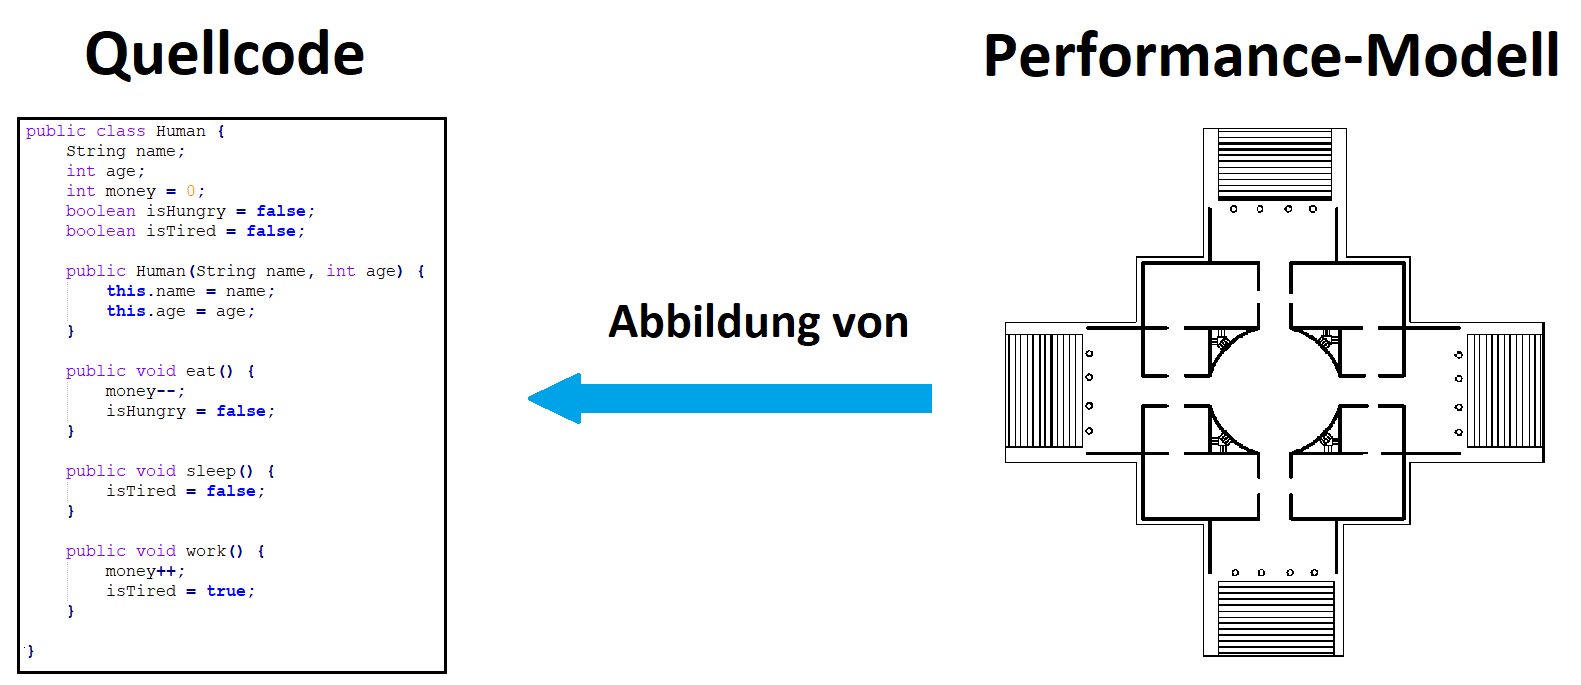
\includegraphics[scale=0.3]{pictures/Abbildung von.png}
%%\caption{Modellbasierte DevOps-Pipeline mit dem CIPM-Ansatz, Quelle: \textcite{mazkatli2020}}
%\end{figure}
%\end{frame}


\begin{frame}{Motivation}
\begin{figure}
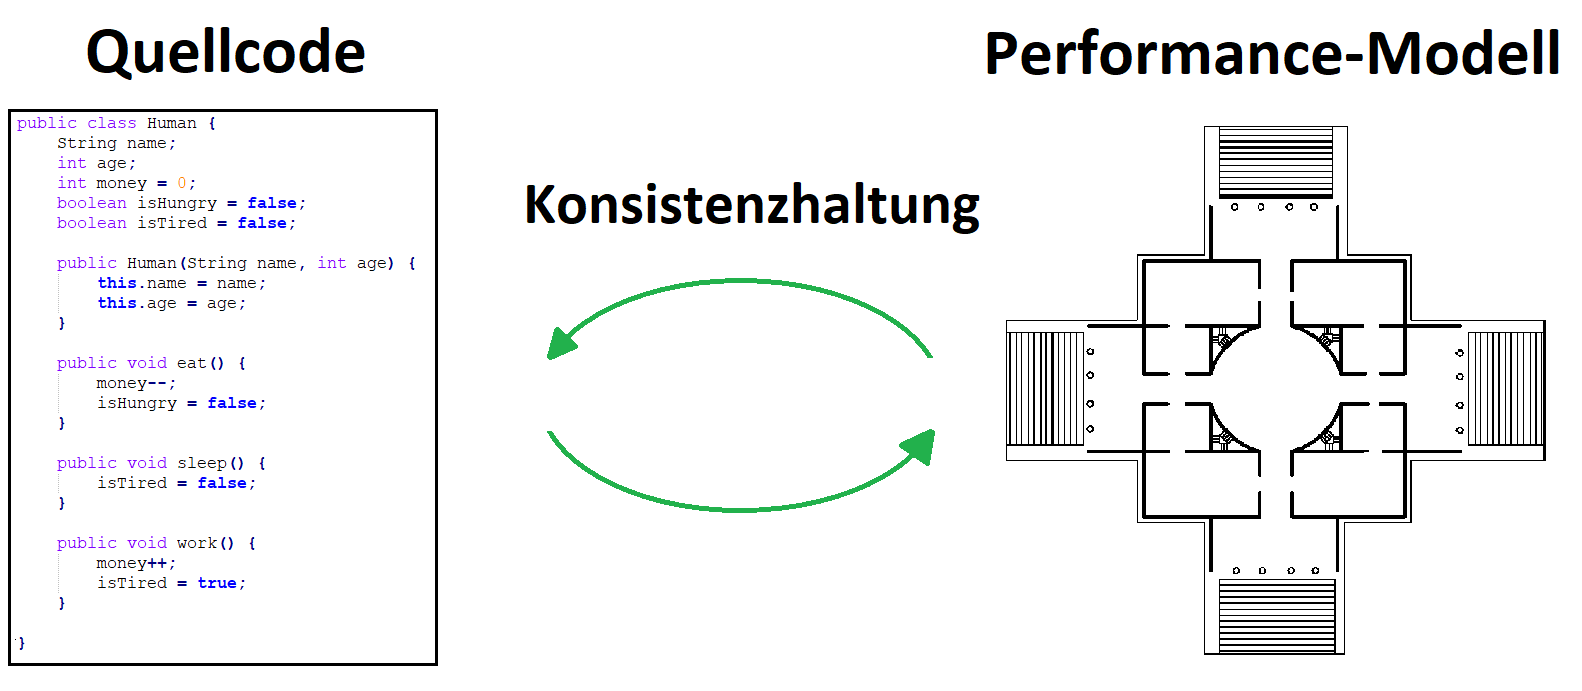
\includegraphics[scale=0.3]{pictures/Konsistenzhaltung.png}
%\caption{Modellbasierte DevOps-Pipeline mit dem CIPM-Ansatz, Quelle: \textcite{mazkatli2020}}
\end{figure}
\end{frame}


%\begin{frame}{PIBA}
%\begin{itemize}
%	\item Problem
%	\begin{itemize}
%		\item CIPM unterstützt keine Continuous Integration
%		\begin{itemize}
%			\item Änderungen im Quellcode werden nicht verfolgt $\Rightarrow$
%			\item Keine automatische inkrementelle Aktualisierung von Performance-Modellen möglich 
%		\end{itemize}				
%	\end{itemize}
%	\item Idee
%	\begin{itemize}
%		\item  Code-Änderungen nach jedem Integrationszyklus lesen und die betroffenen Code-Modelle anpassen  
%	\end{itemize}
%	\item Vorteil
%	\begin{itemize}
%		\item CIPM unterstützt Continuous Integration
%		\begin{itemize}
%			\item CIPM kann in einen agilen Software-Entwicklungsprozess eingebunden werden
%			\item Performance-Modelle werden nach jedem Integrationszyklus automatisch  aktualisiert
%		\end{itemize}
%	\end{itemize}
%	\item Aktionen 
%	\begin{itemize}
%		\item Commit lesen
%		\item Code-Änderungen extrahieren
%		\item Die von den Änderungen betroffenen Code-Modelle anpassen
%	\end{itemize}
%\end{itemize} 
%\end{frame}


\section{Motivation}
\begin{frame}{Motivation: Continuous Integration of
Performance Models (CIPM)}
\begin{figure}
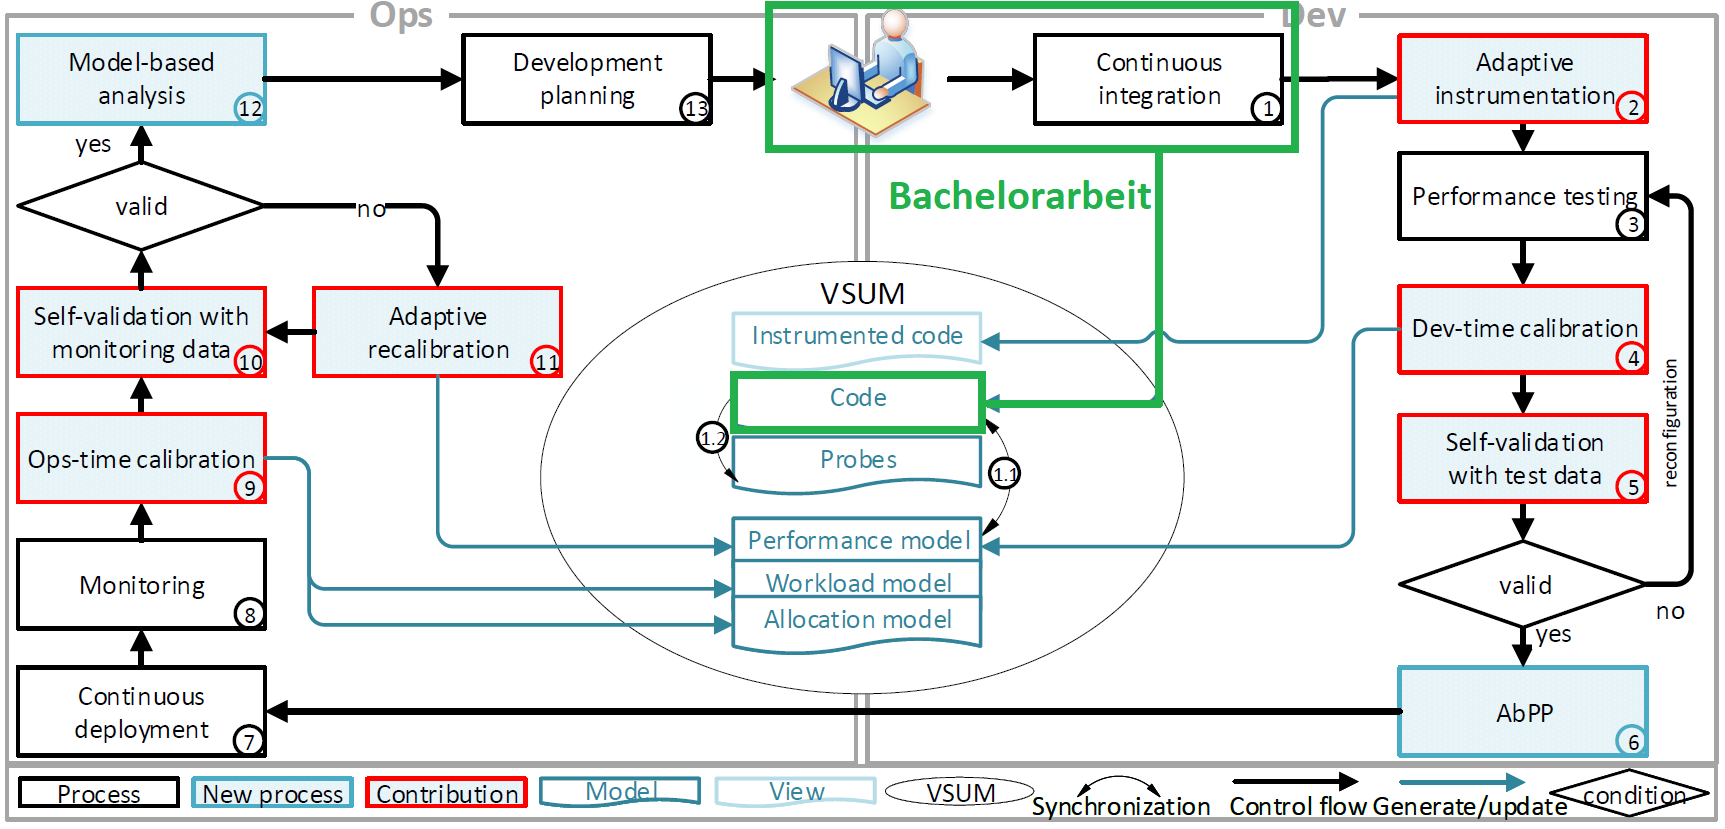
\includegraphics[scale=0.3]{pictures/CIPM in DevOps unser Teil markiert.png}
\caption{Modellbasierte DevOps-Pipeline mit dem CIPM-Ansatz, Quelle: \textcite{mazkatli2020}}
\end{figure}
\end{frame}


%\section{Grundlagen}
%\begin{frame}{Grundlagen}
%\begin{floatingfigure}[r]{9cm}
%\mbox{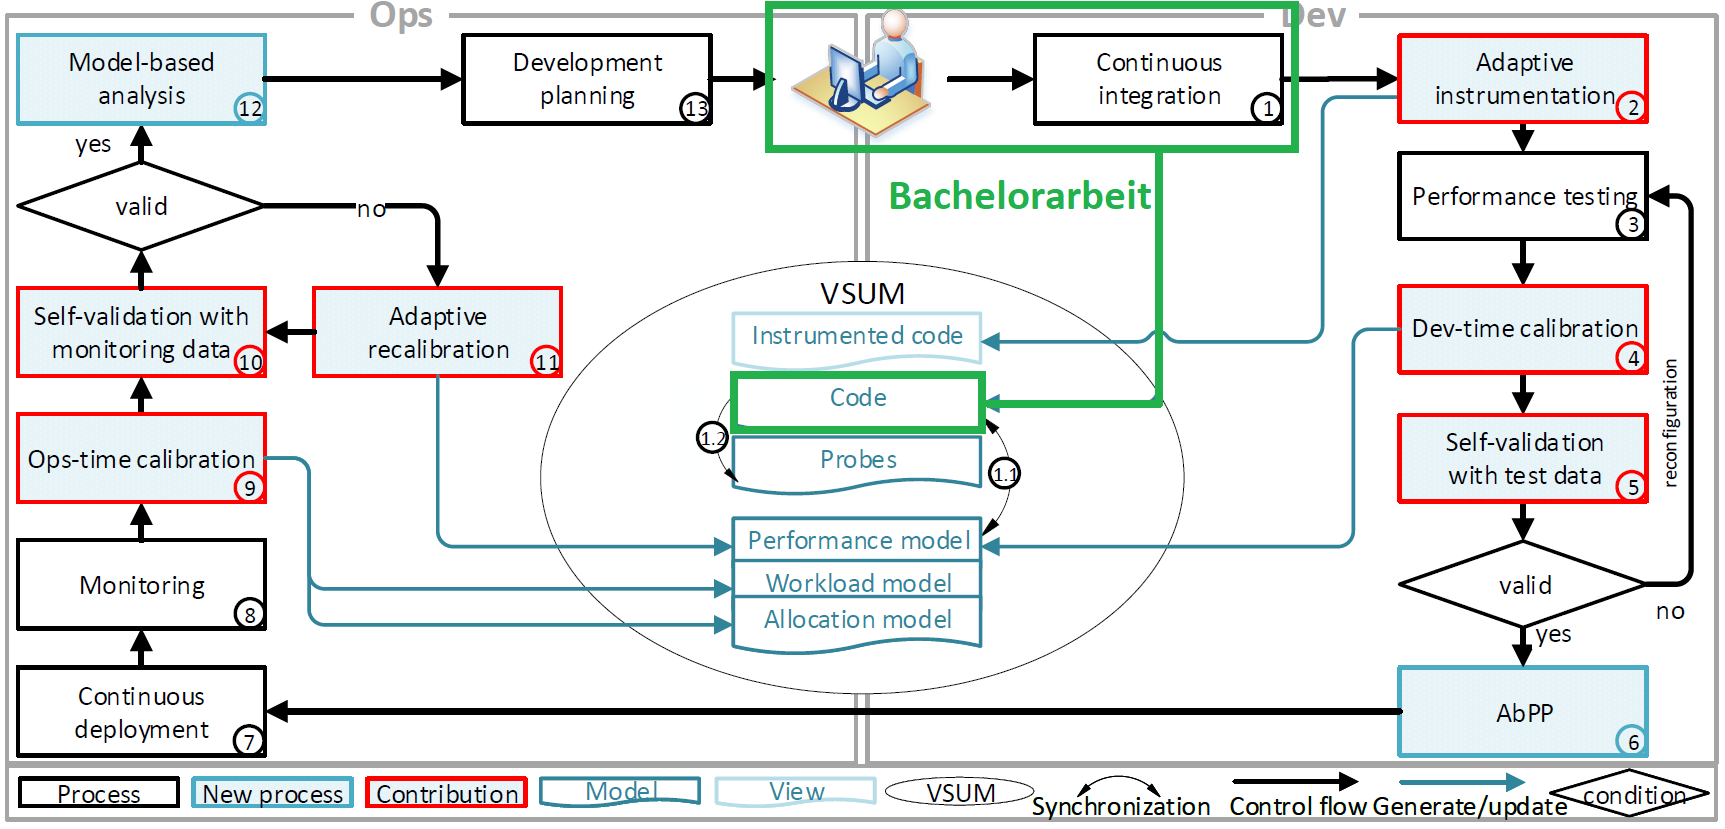
\includegraphics[width=80mm,height=61mm]{pictures/CIPM in DevOps unser Teil markiert.png}}
%\caption{Modellbasierte DevOps-Pipeline, Quelle: \textcite{mazkatli2020}}
%\end{floatingfigure}
%\begin{itemize}
%	\item JGit \cite{jgit}
%	\item Palladio Component Model (PCM) \cite{reussner2016}
%	\item Java Model Parser and Printer (JaMoPP) \cite{jamopp}
%	\item Vitruvius \cite{vitruvius}
%	\item Software Product Line evolution (SPLevo) \cite{splevo}
%	\item EMF Compare \cite{emfcompare}
%\end{itemize}
%\end{frame}


%\begin{frame}{Grundlagen: Tools}
%\begin{itemize}
%	\item JGit \cite{jgit}
%	\begin{itemize}
%		\item JGit repräsentiert ein Git Repository und behandelt Commits
%	\end{itemize}
%
%	\item Palladio Component Model (PCM) \cite{reussner2016}
%	\begin{itemize}
%		\item Palladio Component Model dient als Performance-Modell
%	\end{itemize}
%	\item Java Model Parser and Printer (JaMoPP) \cite{jamopp}
%	\begin{itemize}
%		\item JaMoPP-Modell dient als Java-Quellcode-Modell
%	\end{itemize}
%	\item Vitruvius \cite{vitruvius}
%	\begin{itemize}
%		\item Vitruvius hält alle Modelle konsistent
%	\end{itemize}
%	\item Software Product Line evolution (SPLevo) \cite{splevo}
%	\begin{itemize}
%		\item SPLevo vergleicht JaMoPP-Modelle und ermittelt ihre Differenzen 
%	\end{itemize}
%	\item EMF Compare \cite{emfcompare}
%	\begin{itemize}
%		\item EMF Compare vergleicht EMF-Modelle und ermittelt ihre Differenzen
%	\end{itemize}
%\end{itemize}
%\end{frame}


%\begin{frame}{Grundlagen}
%\begin{itemize}
%	\begin{itemize}
%		\item GumTree extrahiert atomare Code-Änderungen aus einem Commit
%	\end{itemize}
%	\item Vitruvius \cite{vitruvius}
%	\begin{itemize}
%		\item Vitruvius hält alle Modelle konsistent. In unserem Fall PCM- und JaMoPP-Modelle.
%	\end{itemize}
%	\item Software Product Line evolution (SPLevo) \cite{splevo}
%	\begin{itemize}
%		\item SPLevo vergleicht JaMoPP-Modelle miteinander und ermittelt ihre Differenzen 
%	\end{itemize}
%	\item EMF Compare \cite{emfcompare}
%	\begin{itemize}
%		\item EMF Compare vergleicht EMF-Modelle miteinander und ermittelt ihre Differenzen
%	\end{itemize}
%\end{itemize}
%\end{frame}

%\section{Verwandte Arbeiten}
%\begin{frame}{Verwandte Arbeiten}
%\begin{itemize}
%	\item Automated Coevolution of Source Code
%and Software Architecture Models \cite{langhammer2017}
%	\item Extending an Architecture and Code Co-Evolution Approach to Support Existing Software Projects \cite{petersen2016}
%	\begin{itemize}
%		\item ChangeReplay Tool \cite{changereplay}
%	\end{itemize}	
%	\item Integration of Existing Software Artifacts into a View- and
%Change-Driven Development Approach \cite{leonhardt2015}
%\end{itemize}
%\end{frame}





\section{Lösungsansatz}
\begin{frame}{Lösungsansatz}
\begin{figure}
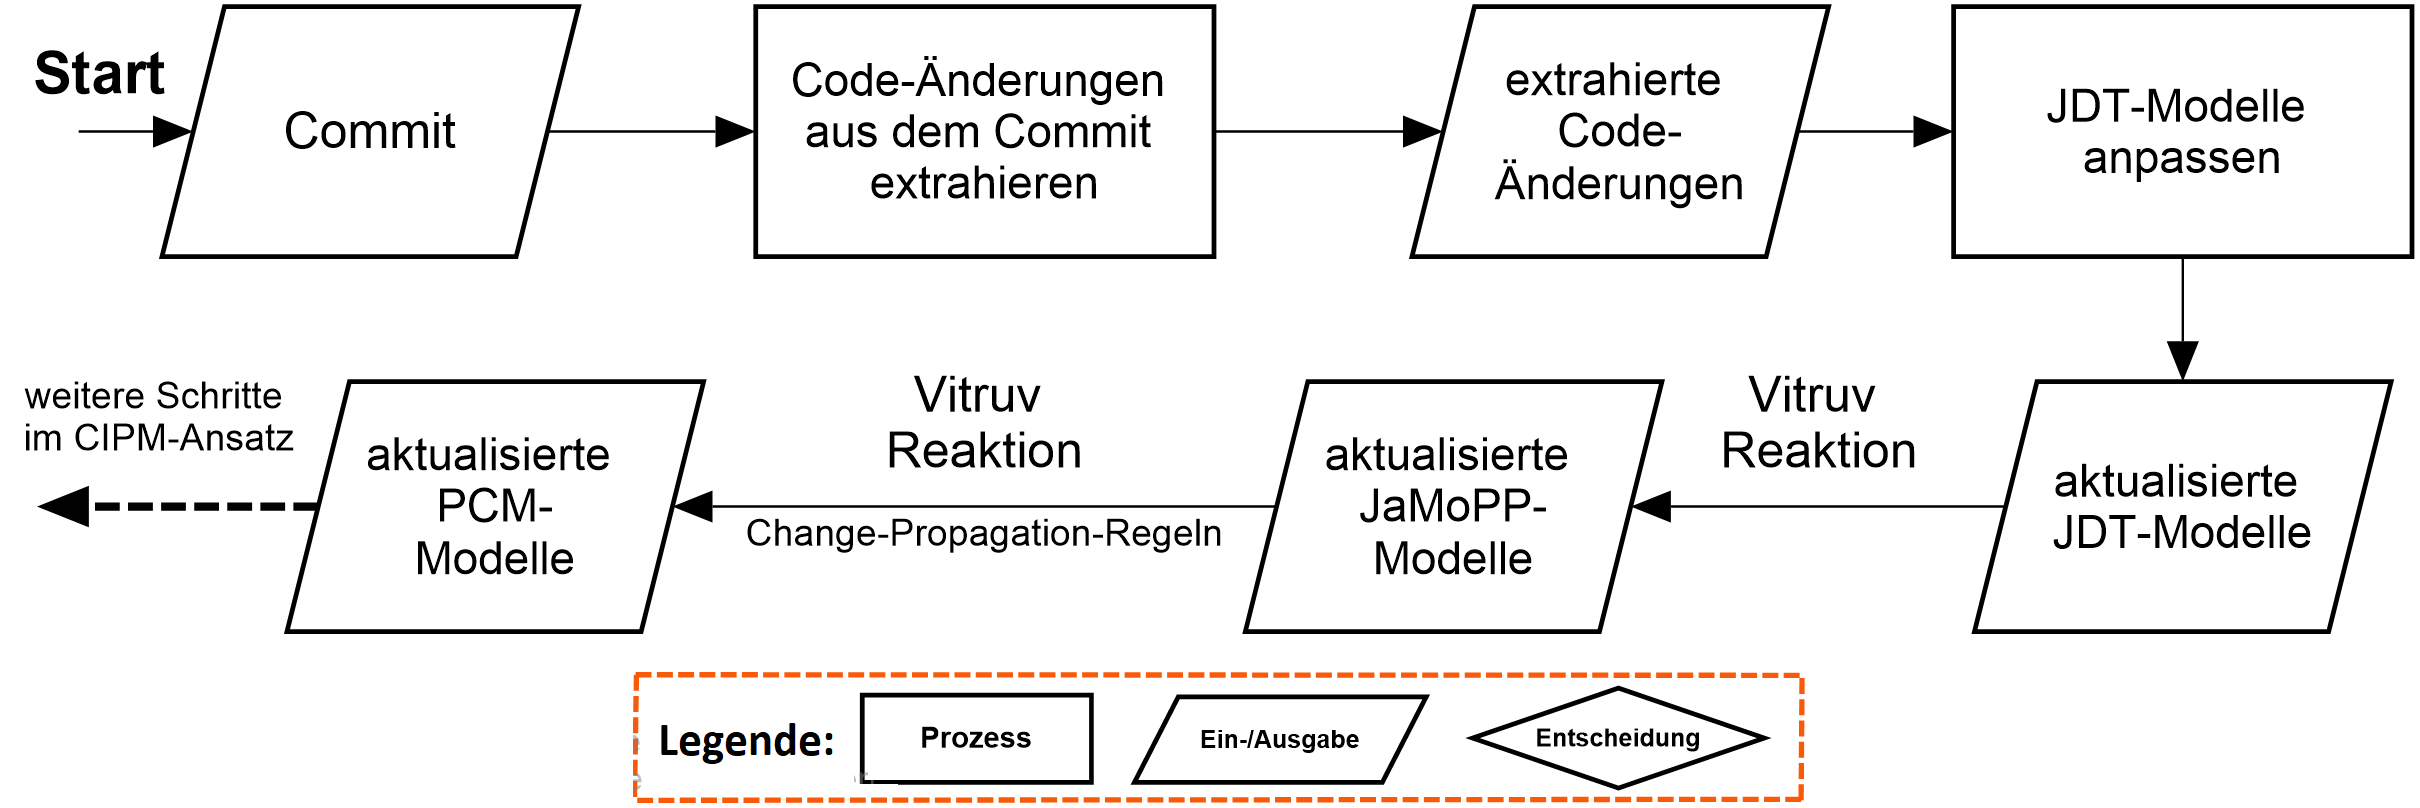
\includegraphics[scale=0.3]{pictures/Vorgehensweise.png}
%\caption{Schritte, die im Rahmen der Bachelorarbeit zu implementieren sind. Ein Rechteck bezeichnet einen Prozess, ein Parallelogramm eine Ein-/Ausgabe}
\end{figure}
\end{frame}


\section{Implementierung}
\begin{frame}{Implementierung: Haupt-Plugin}
\begin{figure}
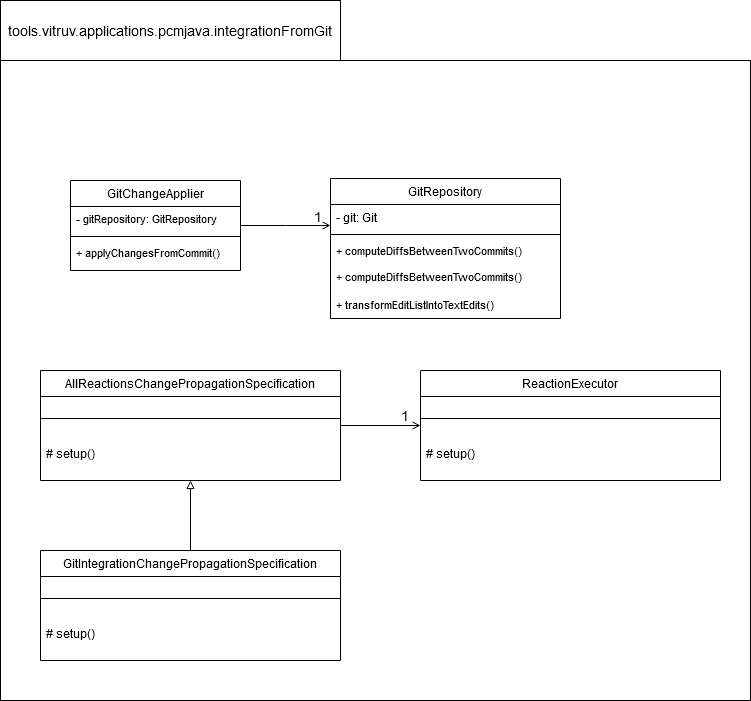
\includegraphics[scale=0.28]{pictures/integrationFromGit_diagram.png}
%\caption{Notwendige Implementierungsschritte für die zweite Strategie. Ein Rechteck bezeichnet einen Prozess, ein Parallelogramm eine Ein-/Ausgabe}
\end{figure}
\end{frame}


\begin{frame}{Implementierung: Test-Plugin}
\begin{figure}
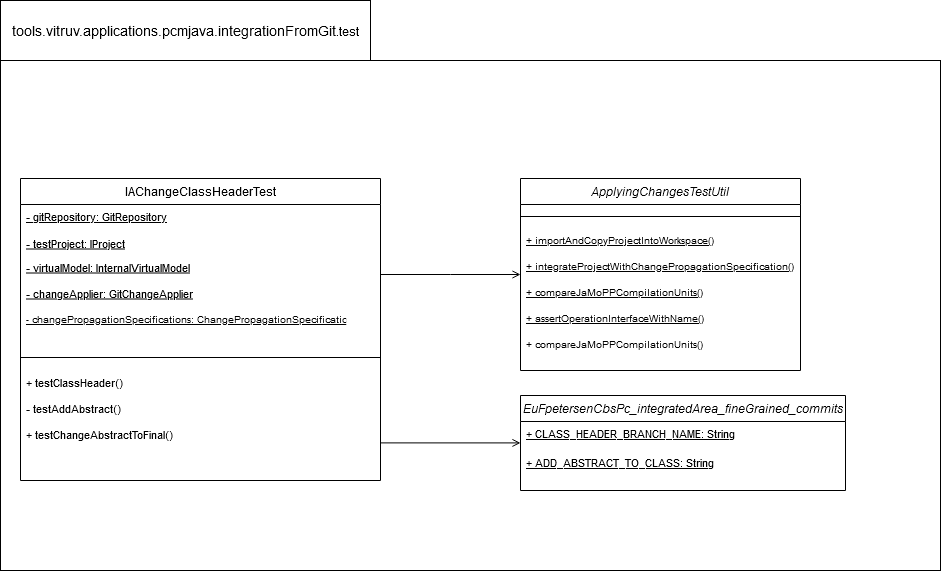
\includegraphics[scale=0.28]{pictures/integrationFromGitTest_diagram.png}
%\caption{Aktualisieren von JaMoPP-Modellen mit Merger}
\end{figure}
\end{frame}


\begin{frame}{Beispieltest: Hinzufügen einer Klassenvariablen}
\begin{figure}
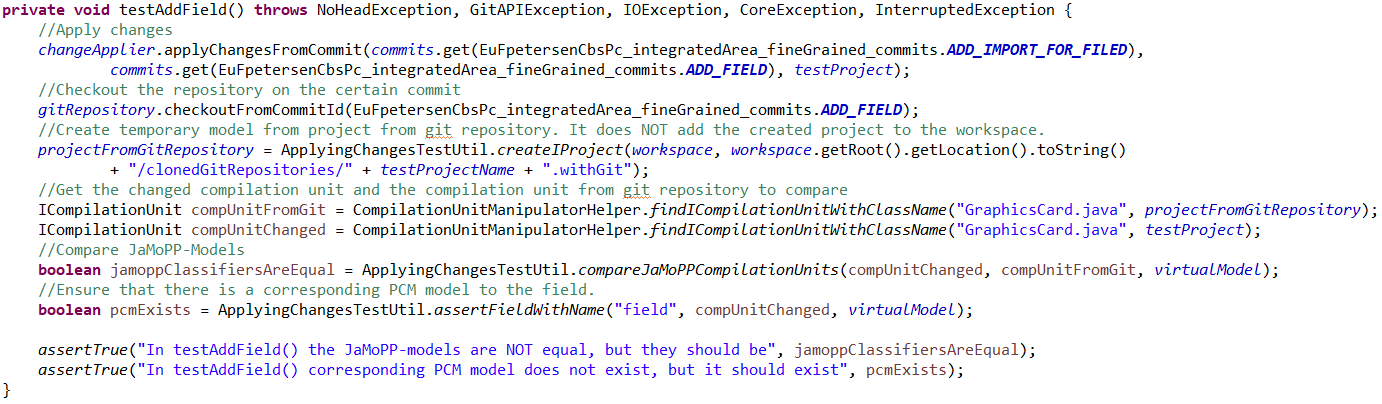
\includegraphics[scale=0.4]{pictures/method_example.png}
%\caption{Notwendige Implementierungsschritte für die dritte Strategie. Ein Rechteck bezeichnet einen Prozess, ein Parallelogramm eine Ein-/Ausgabe}
\end{figure}
\end{frame}

\section{Codereview}
\begin{frame}{Codereview}
\end{frame}

%\begin{frame}{Evaluierung: Aktualisierung der PCM-Modelle}
%\begin{figure}
%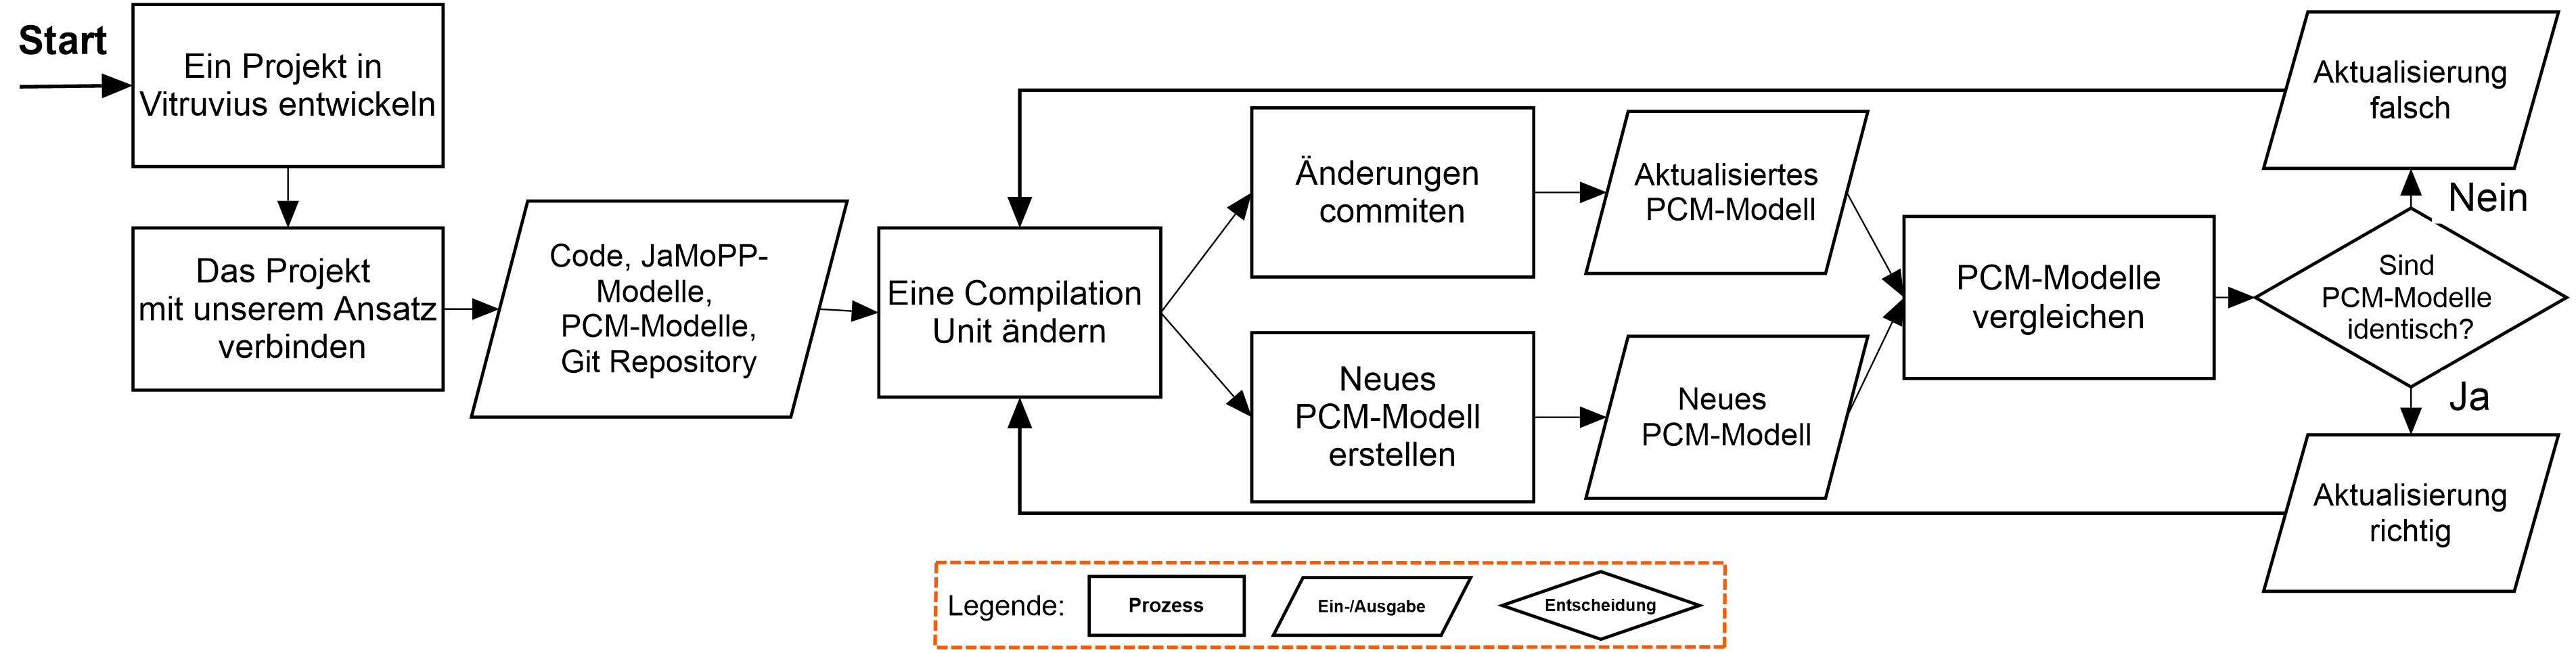
\includegraphics[scale=0.189]{pictures/Evaluierung mit PCM breit Version 3 Teil 2.png}
%%\caption{Evaluierung des implementierten Ansatzes (PCM-Aktualisierung). Ein Rechteck bezeichnet einen Prozess, ein Parallelogramm eine Ein-/Ausgabe, eine Raute eine Entscheidung}
%\end{figure}
%\end{frame}
%
%\section{Arbeitsplan}
%\begin{frame}{Arbeitsplan}
%\begin{figure}
%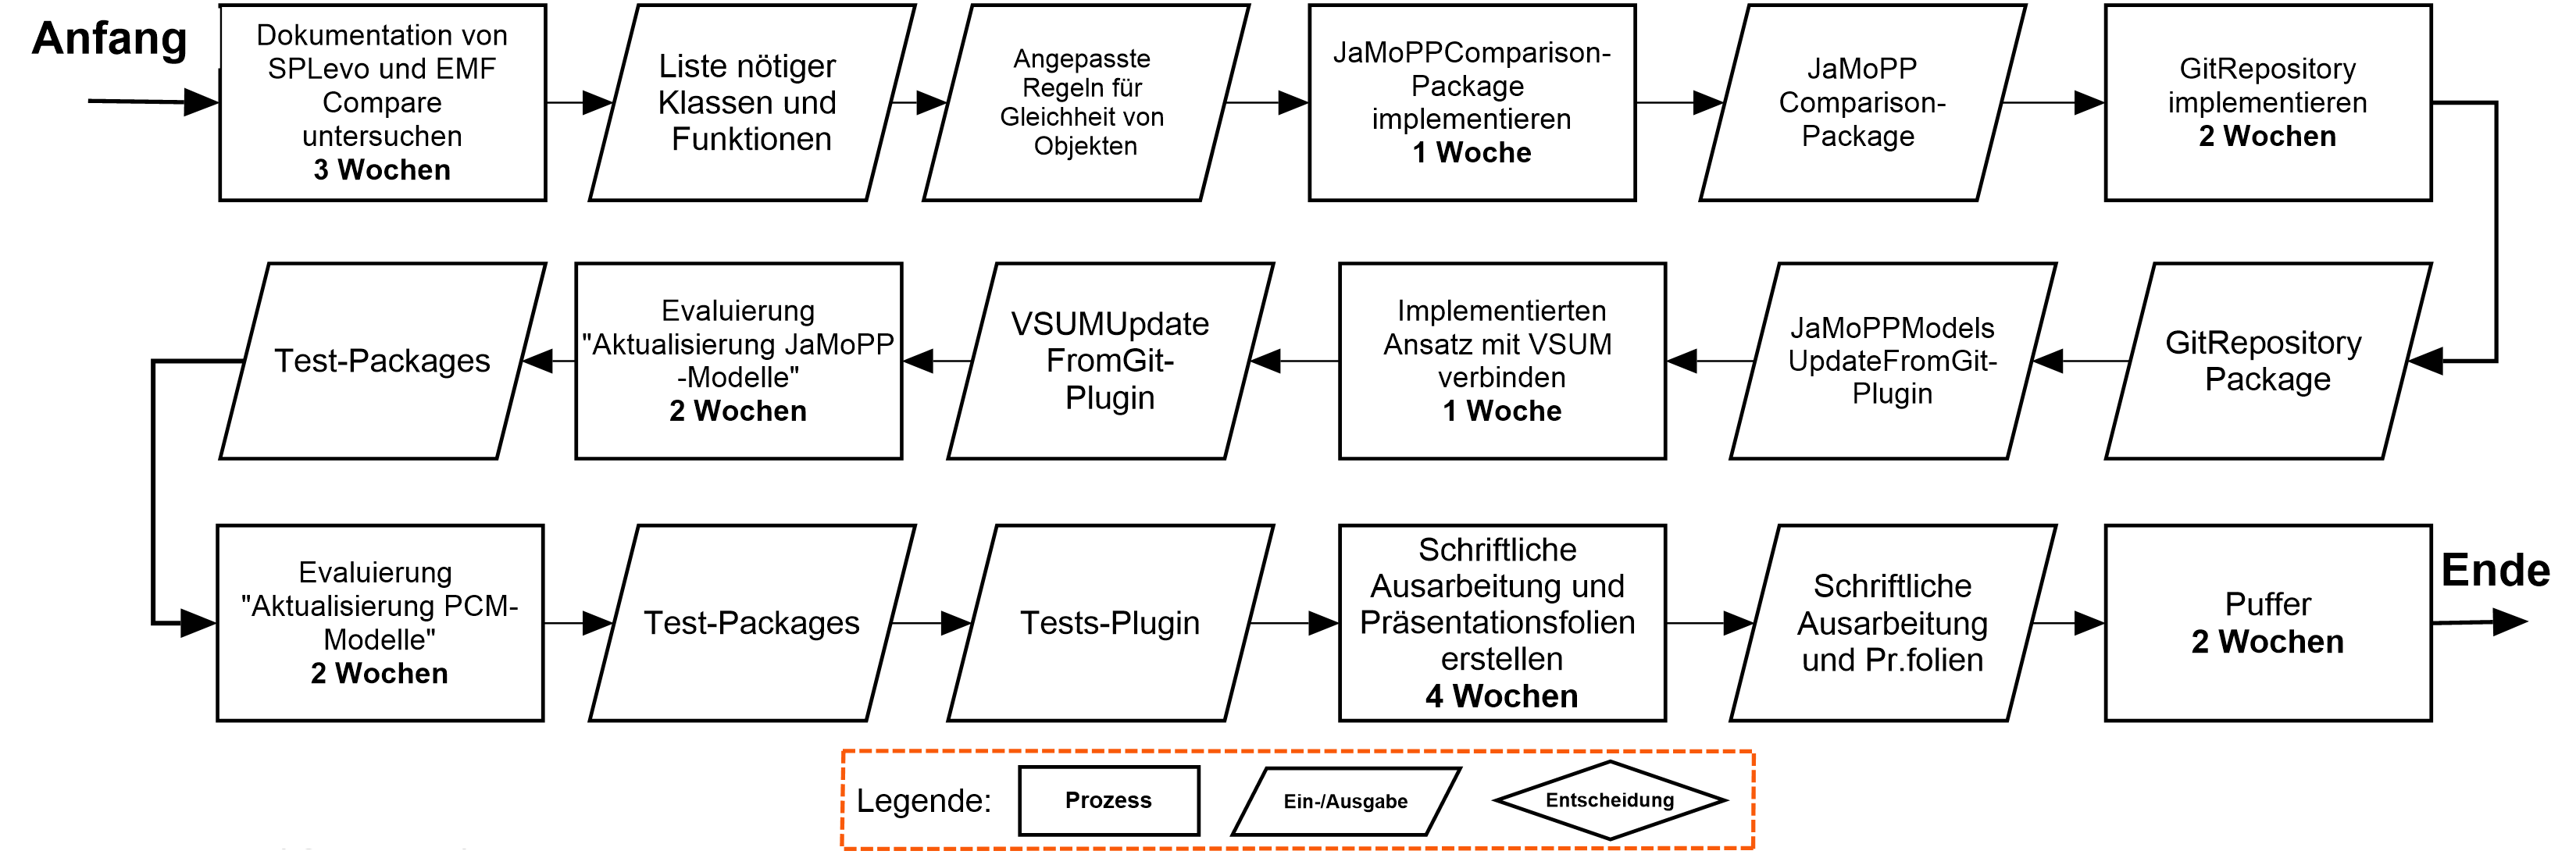
\includegraphics[scale=0.22]{pictures/Zeitplan_Flussdiagramm_breit Version 3.png}
%%\caption{Arbeitsschritte mit Zeitangaben. Ein Rechteck bezeichnet einen Prozess, ein Parallelogramm eine Ein-/Ausgabe, eine Raute eine Entscheidung}
%\end{figure}
%\end{frame}
%
%\section{Zusammenfassung}
%\begin{frame}{Zusammenfassung}
%\begin{itemize}
%	\item Problem
%	\begin{itemize}
%		\item CIPM unterstützt keine Continuous Integration
%		\begin{itemize}
%			\item Änderungen im Quellcode werden nicht verfolgt $\Rightarrow$
%			\item Keine automatische inkrementelle Aktualisierung von Performance-Modellen möglich 
%		\end{itemize}				
%	\end{itemize}
%	\item Idee
%	\begin{itemize}
%		\item  Code-Änderungen nach jedem Integrationszyklus lesen und die betroffenen Code-Modelle anpassen  
%	\end{itemize}
%	\item Vorteil
%	\begin{itemize}
%		\item CIPM unterstützt Continuous Integration
%		\begin{itemize}
%			\item CIPM kann in einen agilen Software-Entwicklungsprozess eingebunden werden
%			\item Performance-Modelle werden nach jedem Integrationszyklus automatisch  aktualisiert
%		\end{itemize}
%	\end{itemize}
%	\item Aktionen 
%	\begin{itemize}
%		\item Commit lesen
%		\item Code-Änderungen extrahieren
%		\item Die von den Änderungen betroffenen Code-Modelle anpassen
%	\end{itemize}
%\end{itemize}  
%\end{frame}

%\appendix
%\beginbackup

%\begin{frame}[allowframebreaks]{References}
\printbibliography
%\end{frame}

%\backupend

\end{document}
